\chapter{System Testing and Evaluation}\label{chap:testingEvaluation}

%\version{v1.11.2015}

\section*{}
\section{Graphical user interface testing}
\begin{figure}[!htb]
	\begin{minipage}{0.48\textwidth}
		\centering
		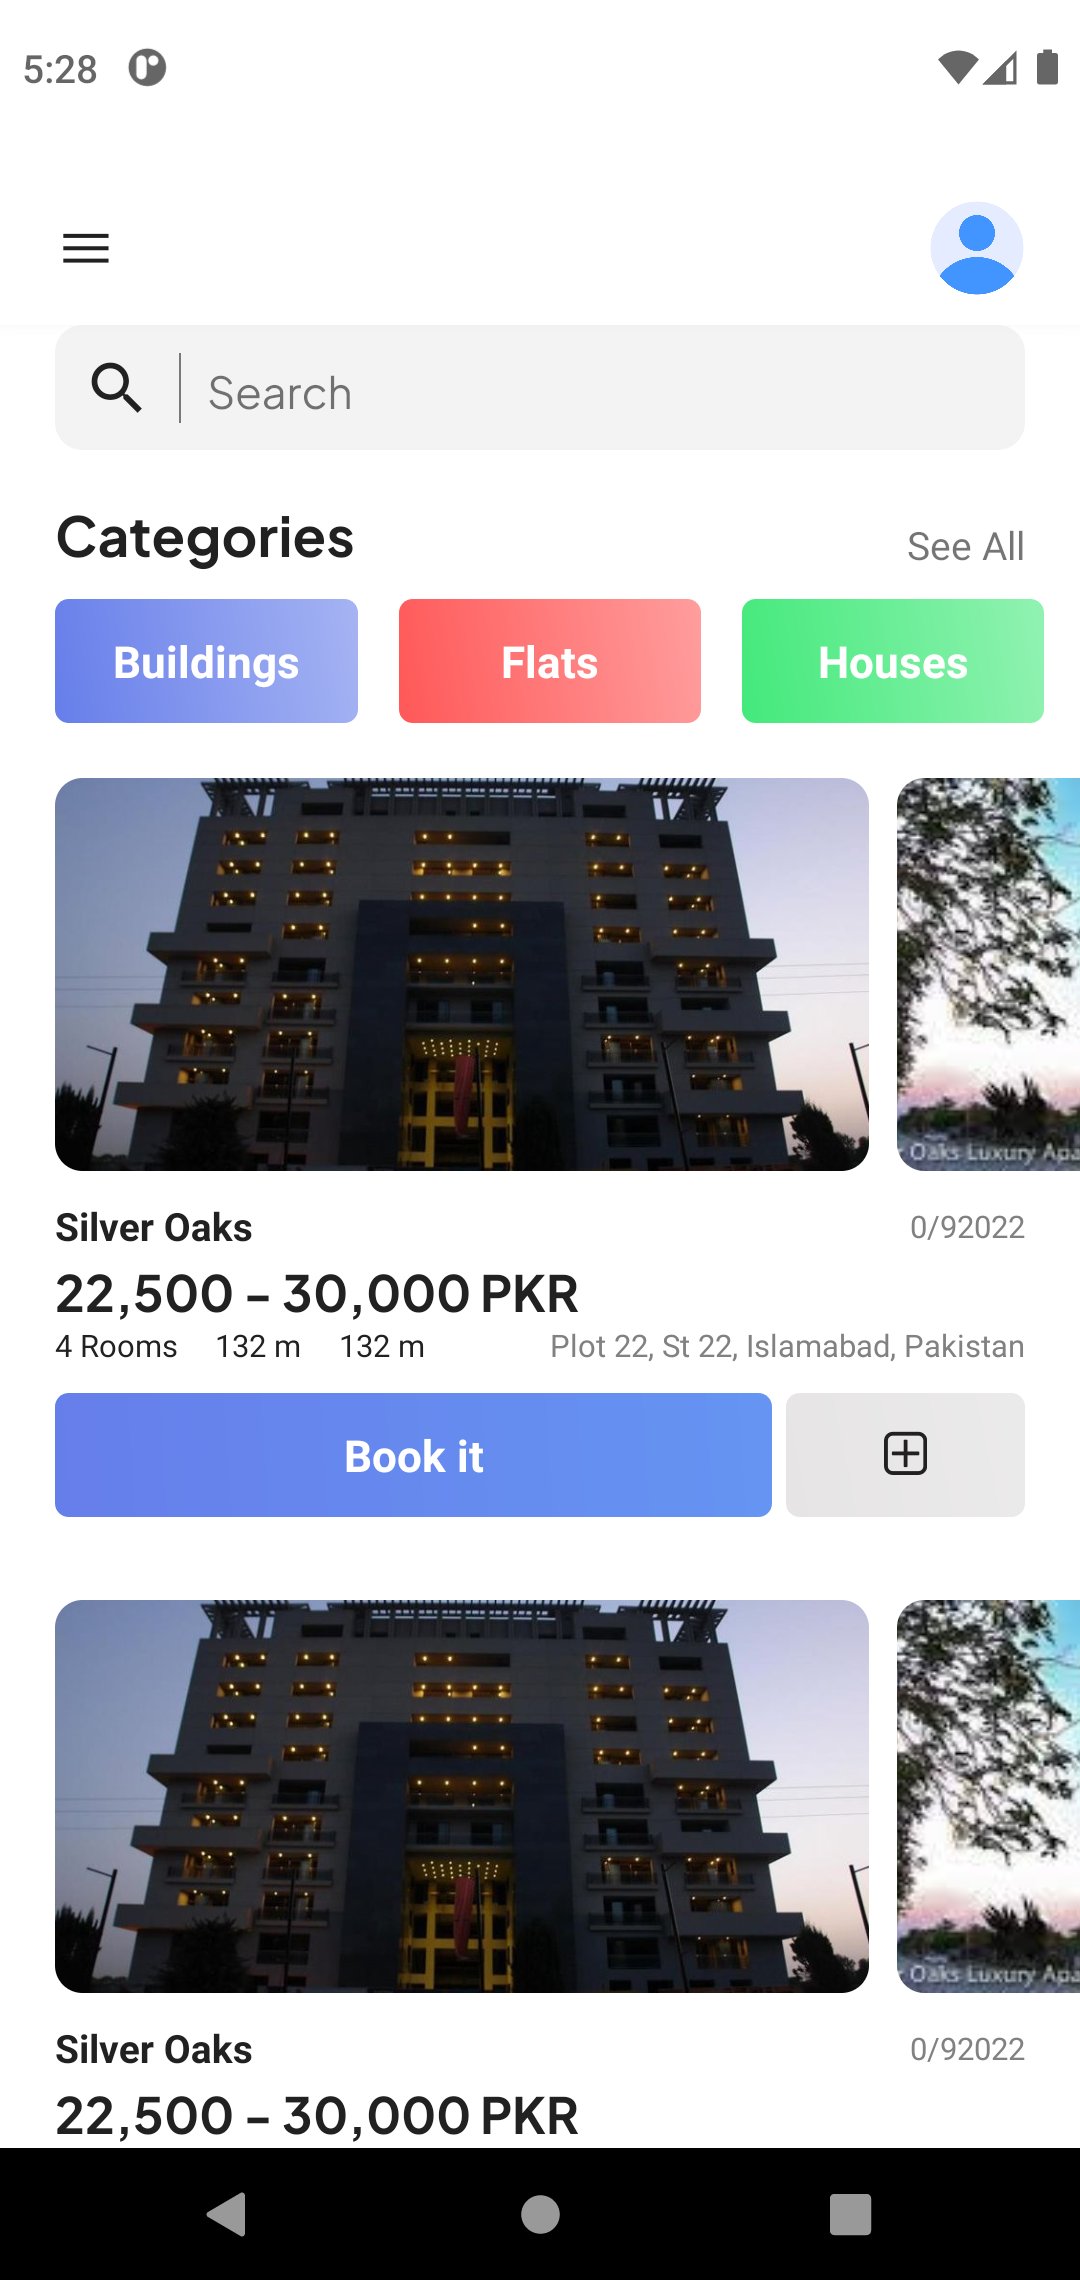
\includegraphics[width=0.7\linewidth]{figures/Testing/scroll1.png}
		\caption{Before Scrolling}\label{Fig:Data1}
	\end{minipage}\hfill
	\begin{minipage}{0.48\textwidth}
		\centering
		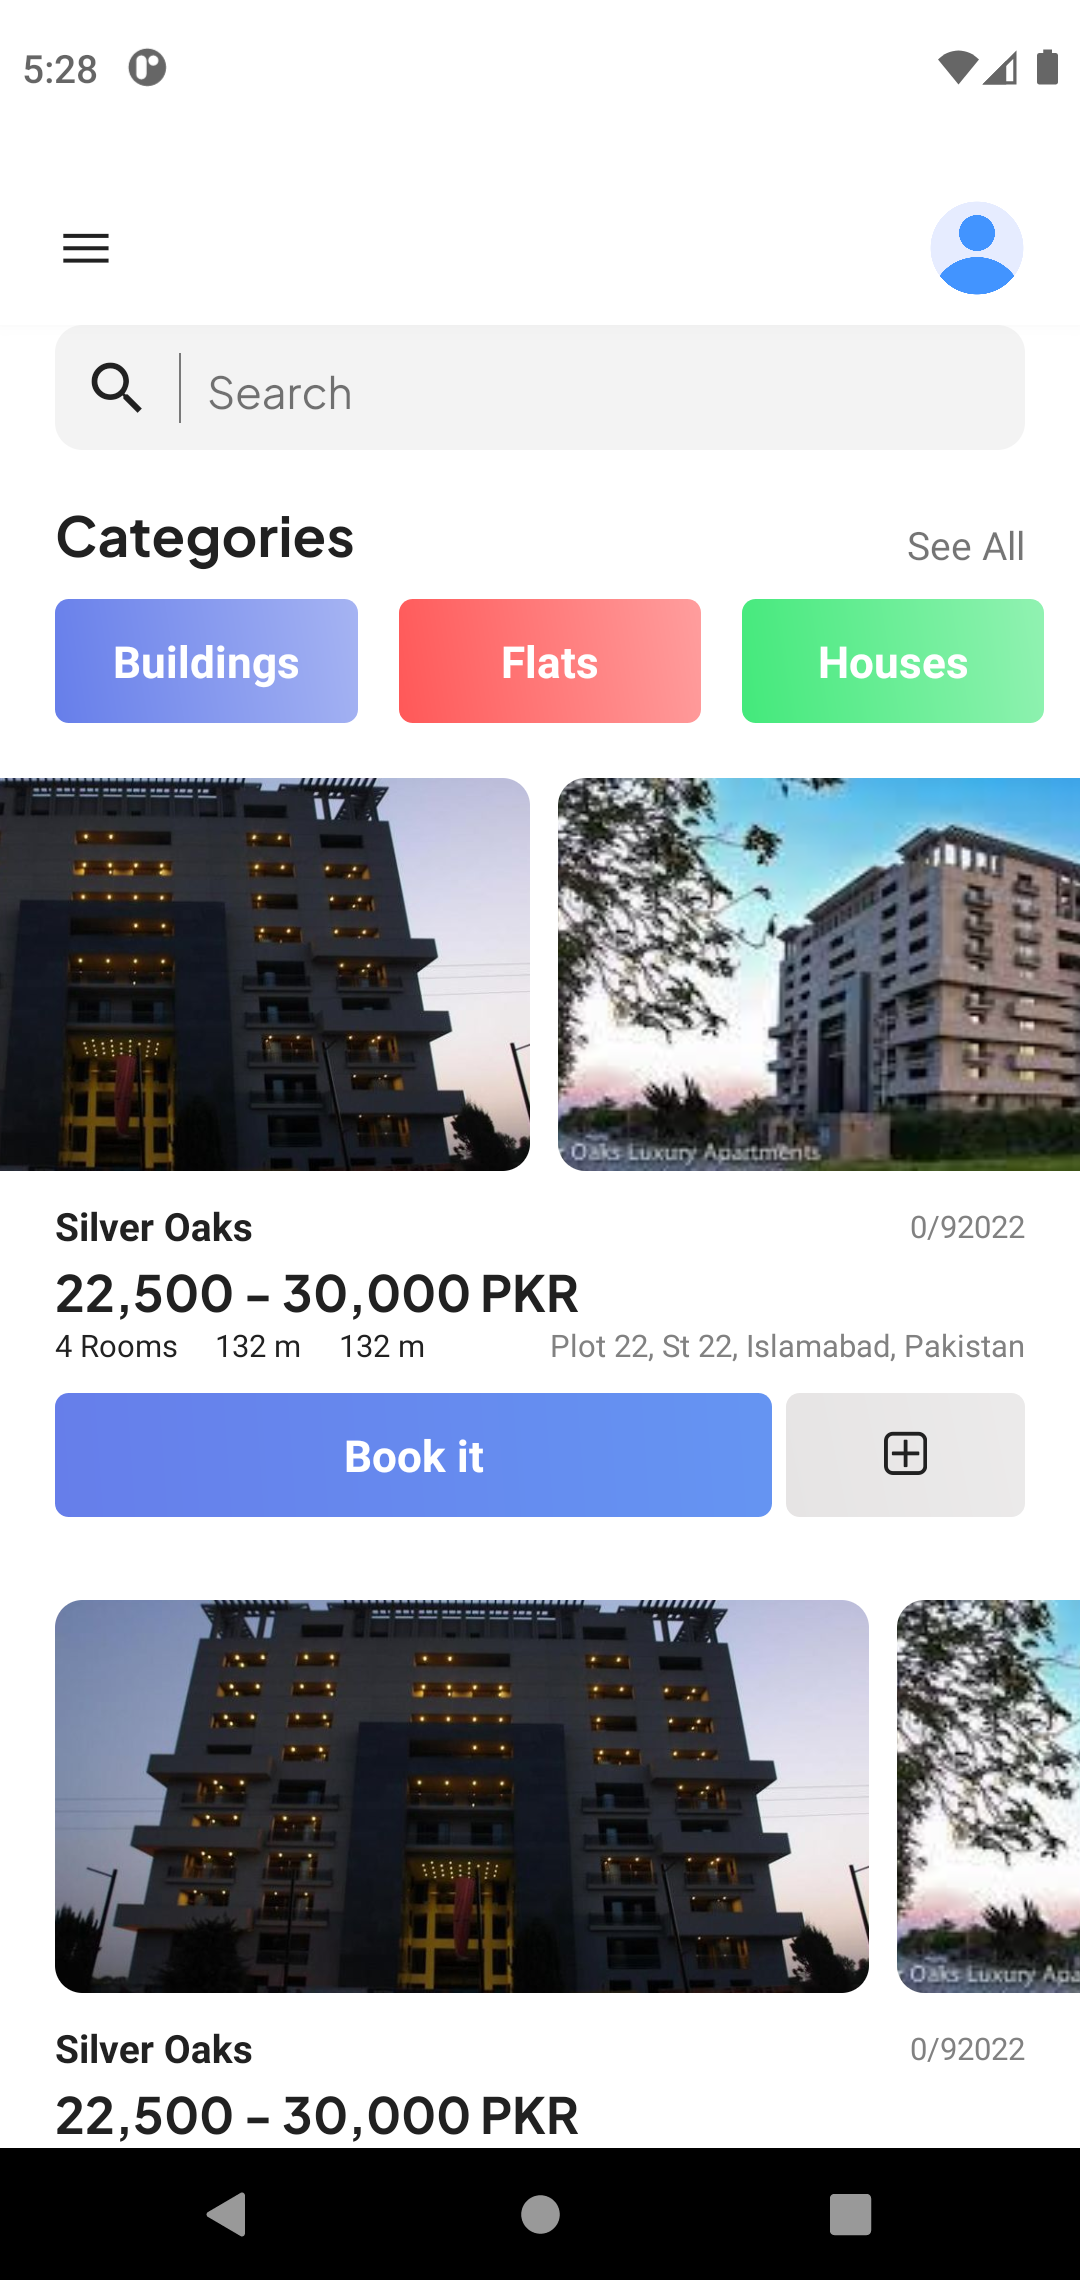
\includegraphics[width=0.7\linewidth]{figures/Testing/scroll2.png}
		\caption{After Scrolling}\label{Fig:Data2}
	\end{minipage}
\end{figure}
While the image scrolls, it does not cut off at the margins but goes through the entire width of the screen which shows successful implementation of the scrolling
\newpage
\begin{figure}[!htb]
	\begin{minipage}{0.48\textwidth}
		\centering
		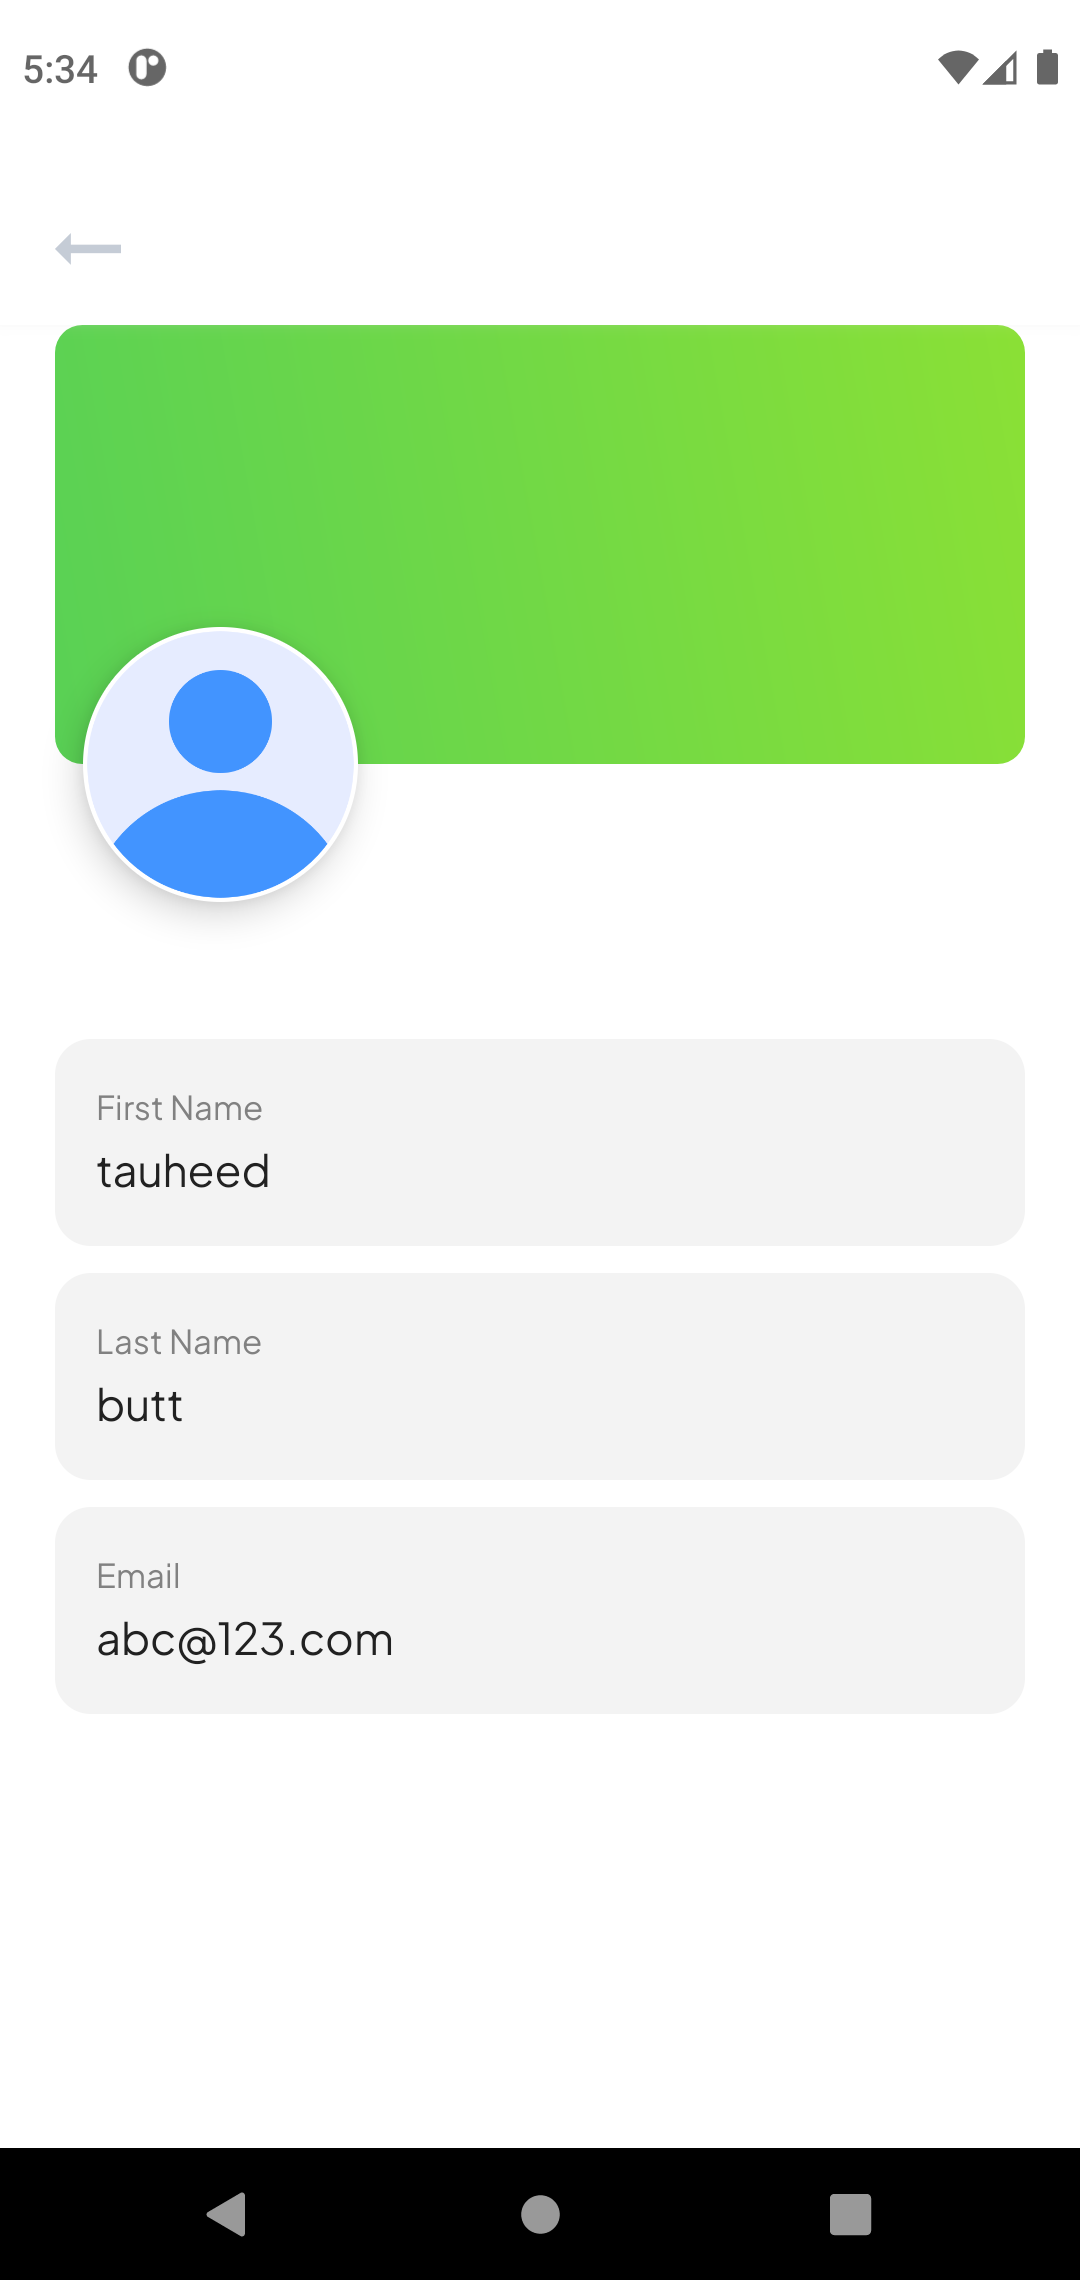
\includegraphics[width=0.8\linewidth]{figures/Testing/change1.png}
		\caption{Before Changing Data}\label{Fig:Data1}
	\end{minipage}\hfill
	\begin{minipage}{0.48\textwidth}
		\centering
		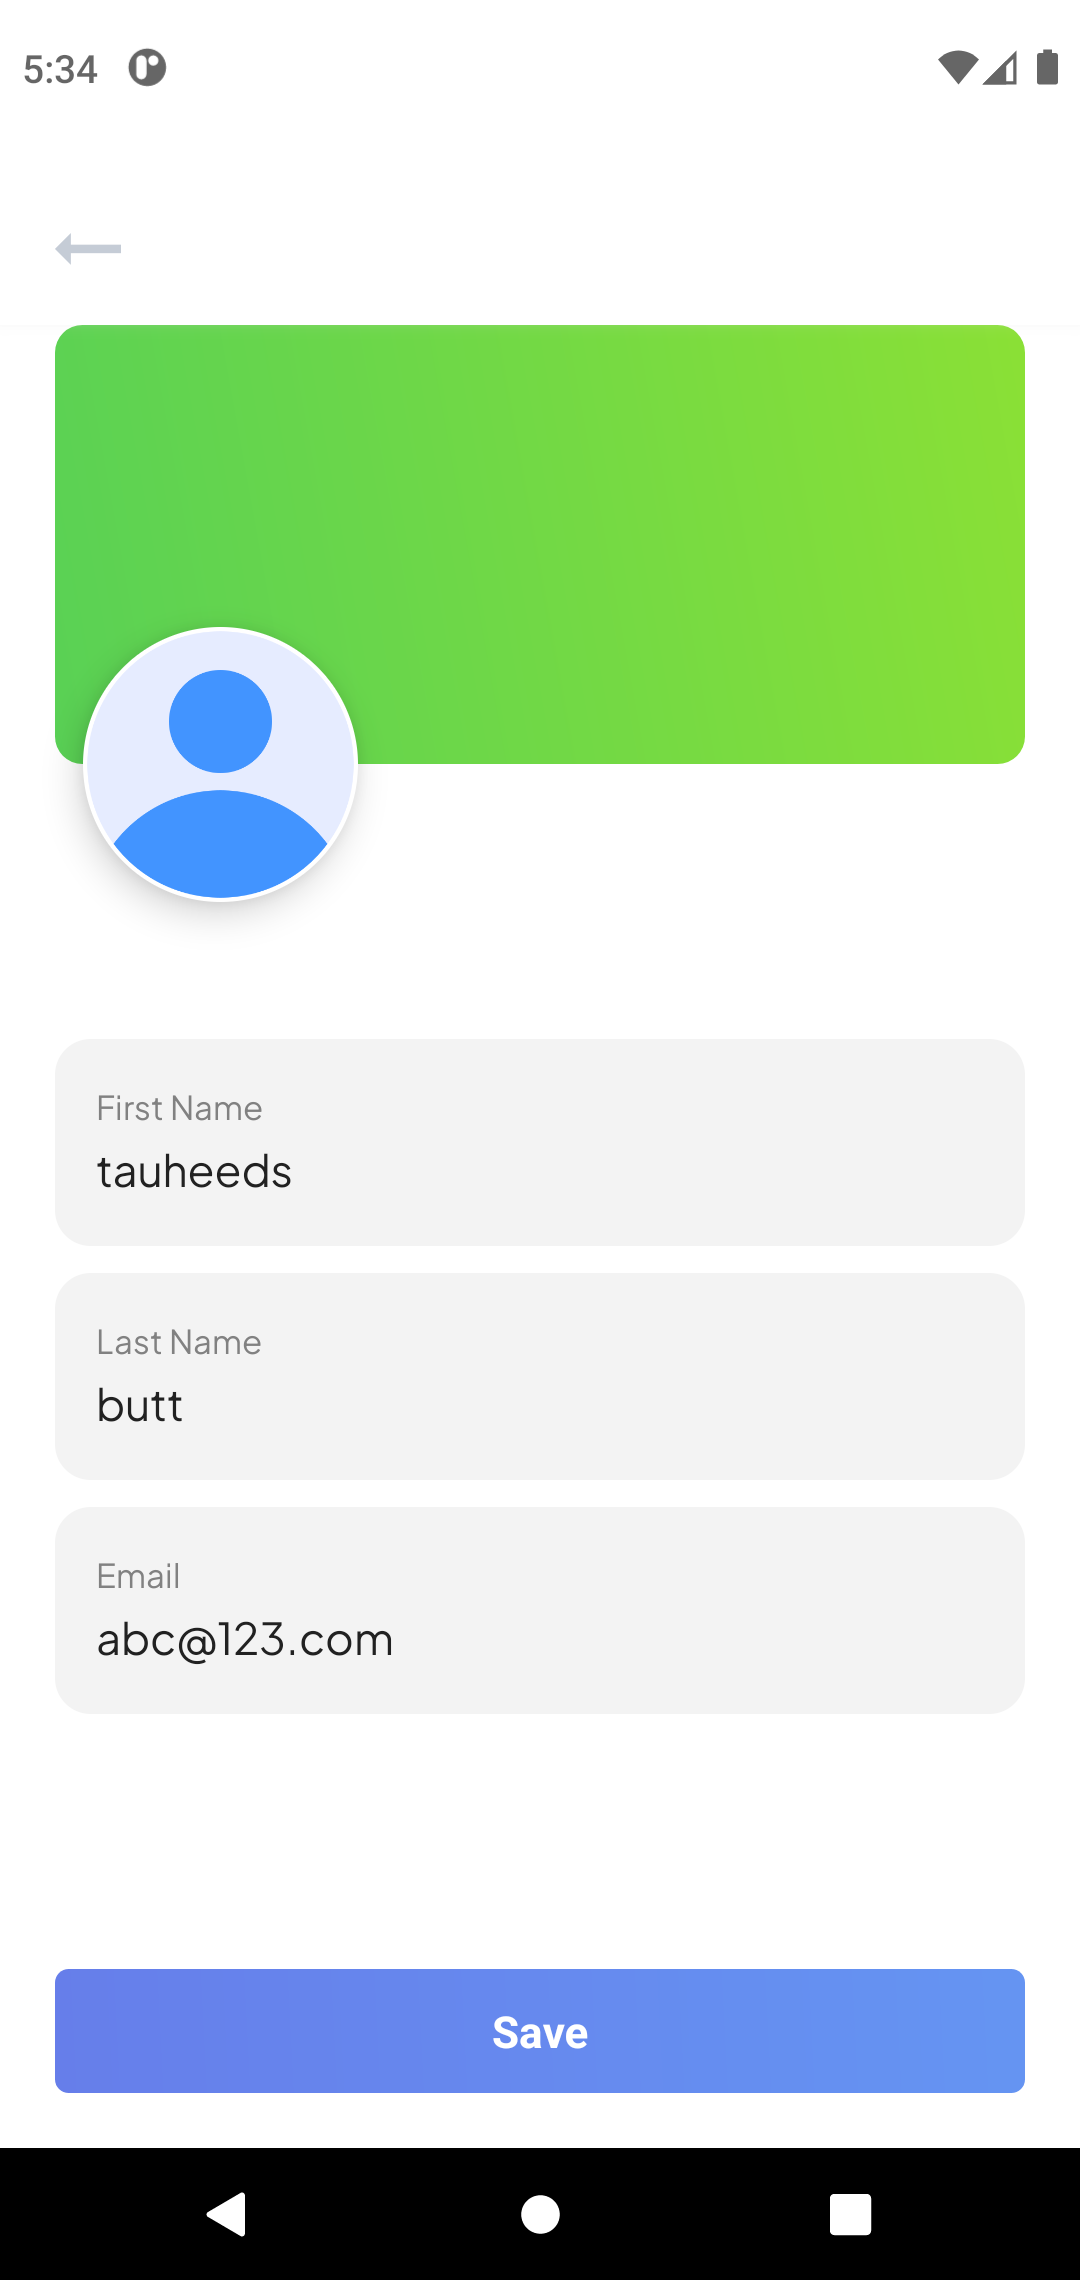
\includegraphics[width=0.8\linewidth]{figures/Testing/change2.png}
		\caption{After Changing Data}\label{Fig:Data2}
	\end{minipage}
\end{figure}
When the User profile is changed, a button shows up to indicate the user to save the changes. if the values are the same, the button goes away.
\newpage
\begin{figure}[!htb]
	\begin{minipage}{0.48\textwidth}
		\centering
		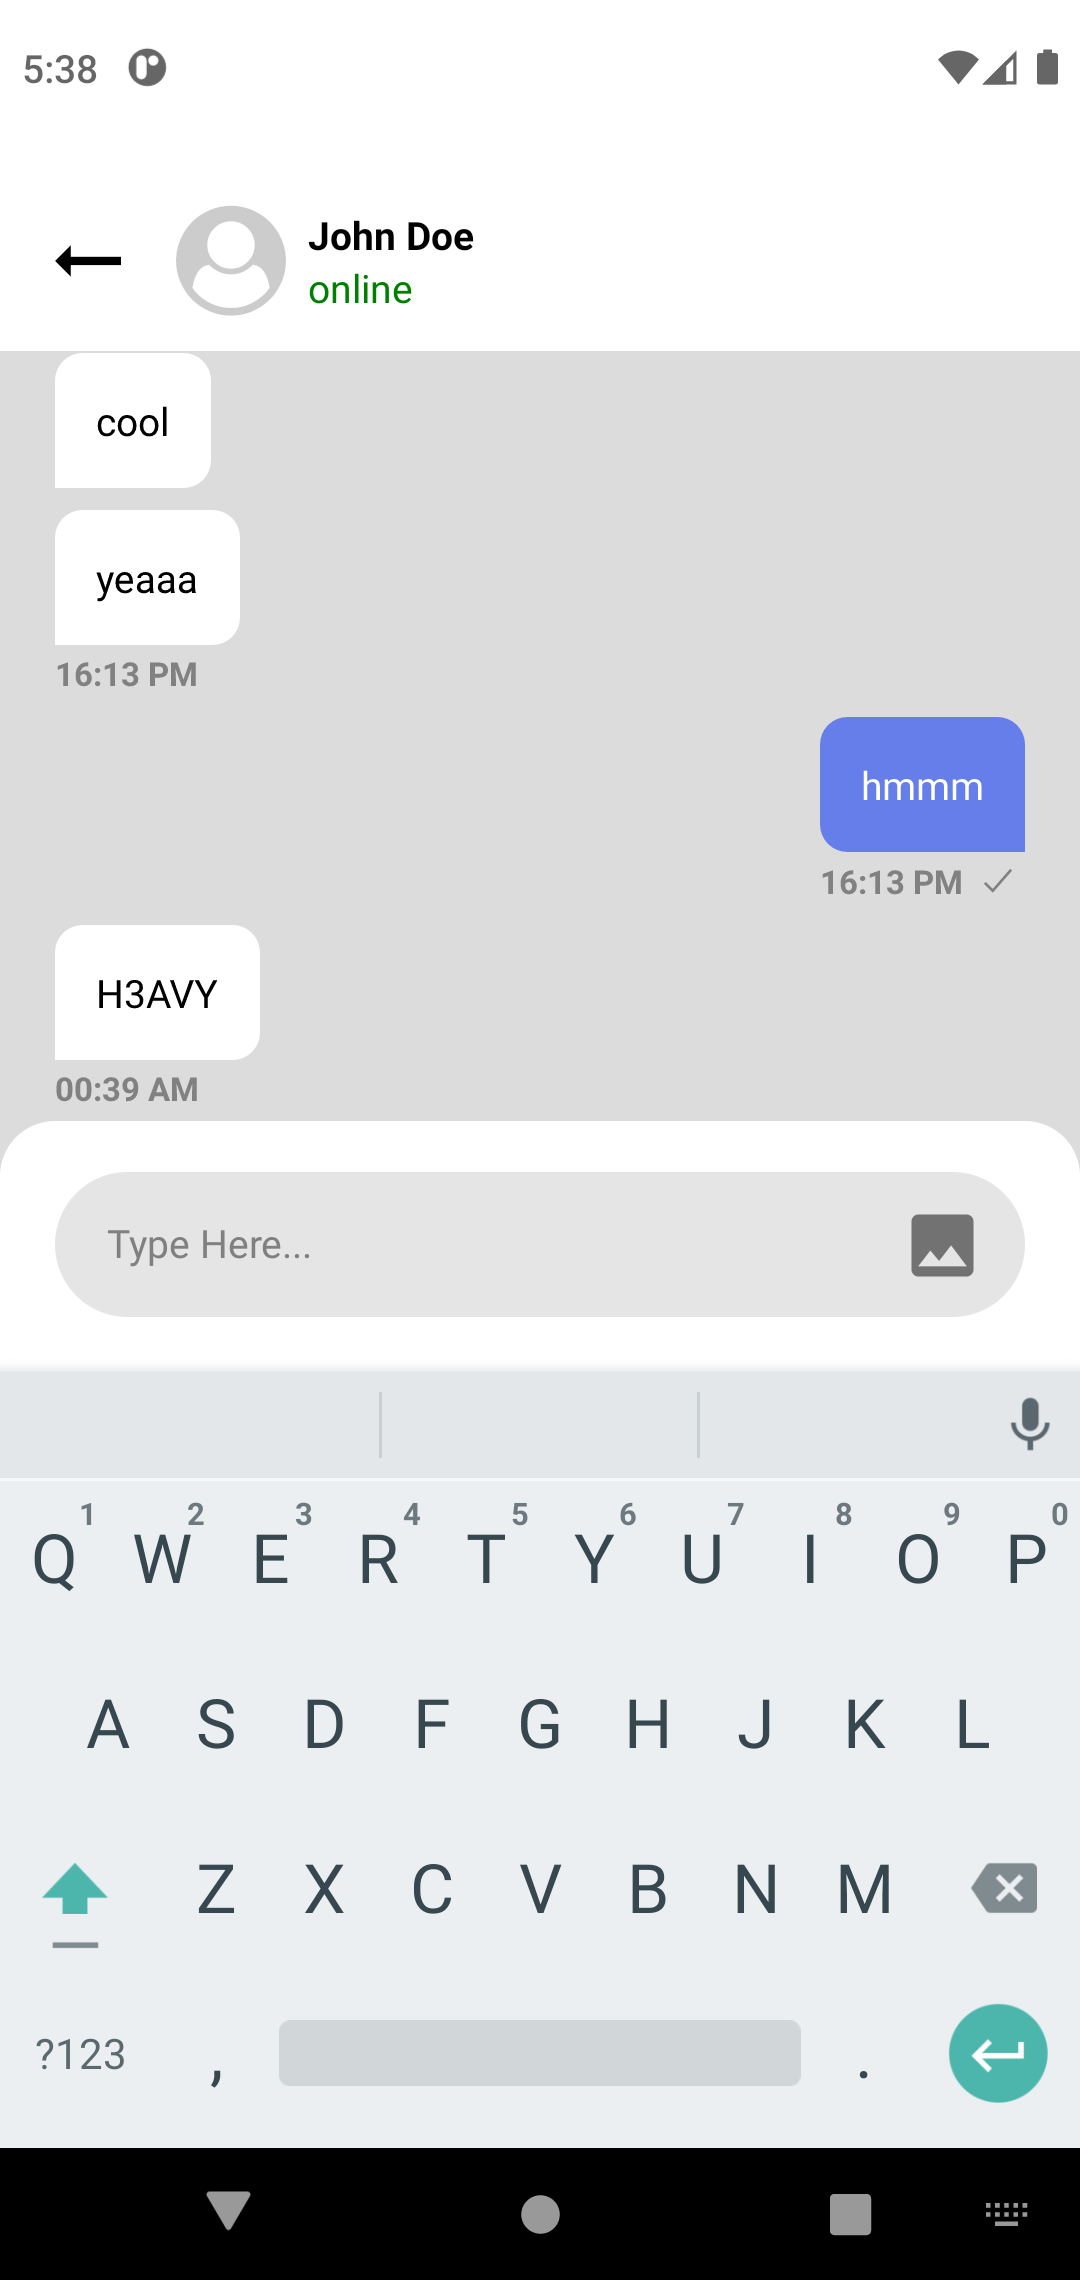
\includegraphics[width=0.8\linewidth]{figures/Testing/chat1.png}
		\caption{Before Typing Message}\label{Fig:Data1}
	\end{minipage}\hfill
	\begin{minipage}{0.48\textwidth}
		\centering
		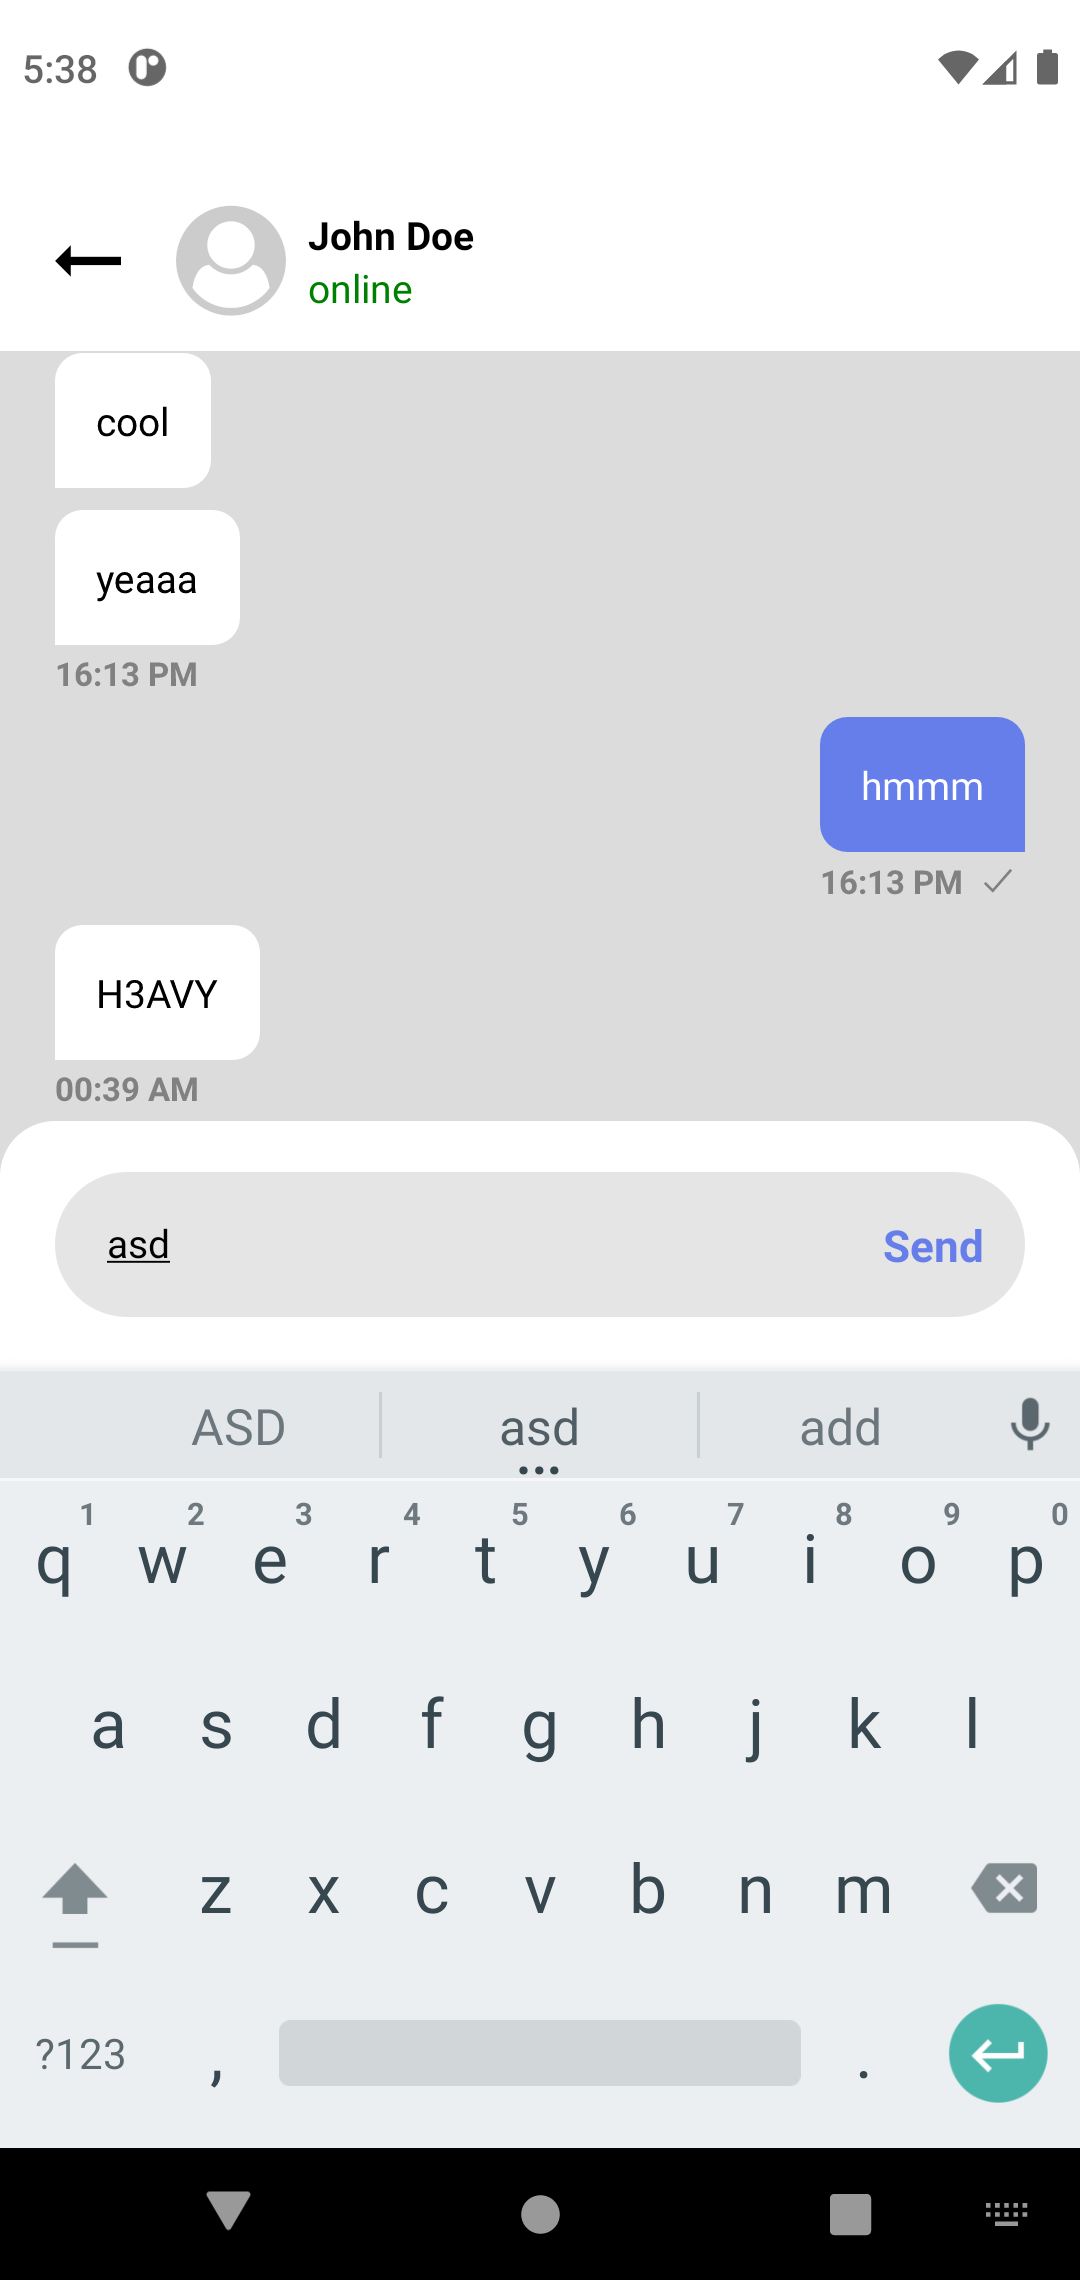
\includegraphics[width=0.8\linewidth]{figures/Testing/chat2.png}
		\caption{After Typing Message}\label{Fig:Data2}
	\end{minipage}
\end{figure}
When a message is typed, only then the SEND button shows. If the box is empty, the gallery button is shown.
\newpage

\begin{figure}[H]
	\centering
	\makebox[\textwidth]{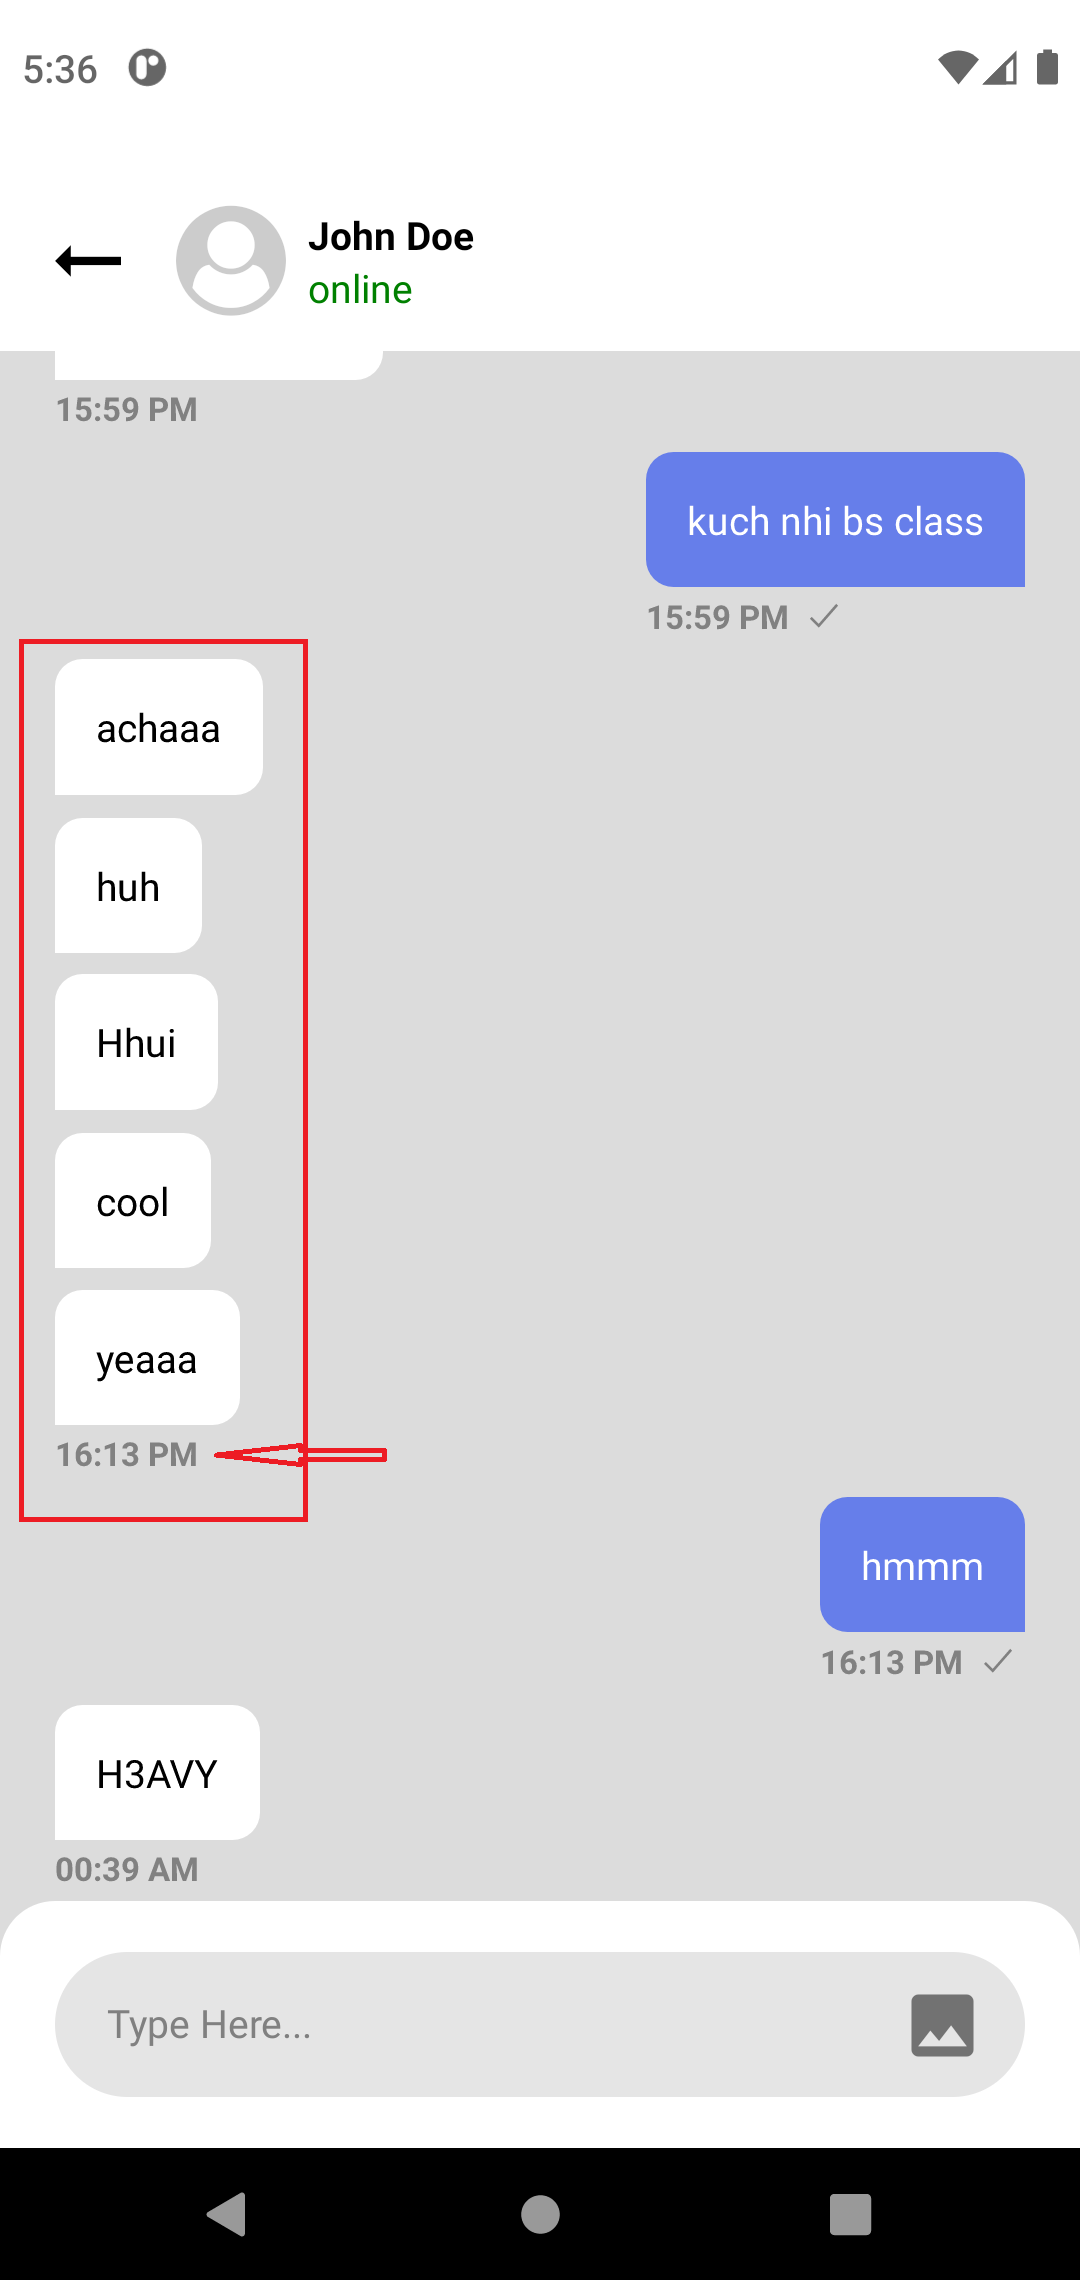
\includegraphics[scale=0.3]{figures/Testing/chat.png}}%
	\caption{Before Typing Message}
\end{figure}
The time the message was sent is only shown at the last message of the user without interruption.

\newpage
\begin{figure}[H]
	\centering
	\makebox[\textwidth]{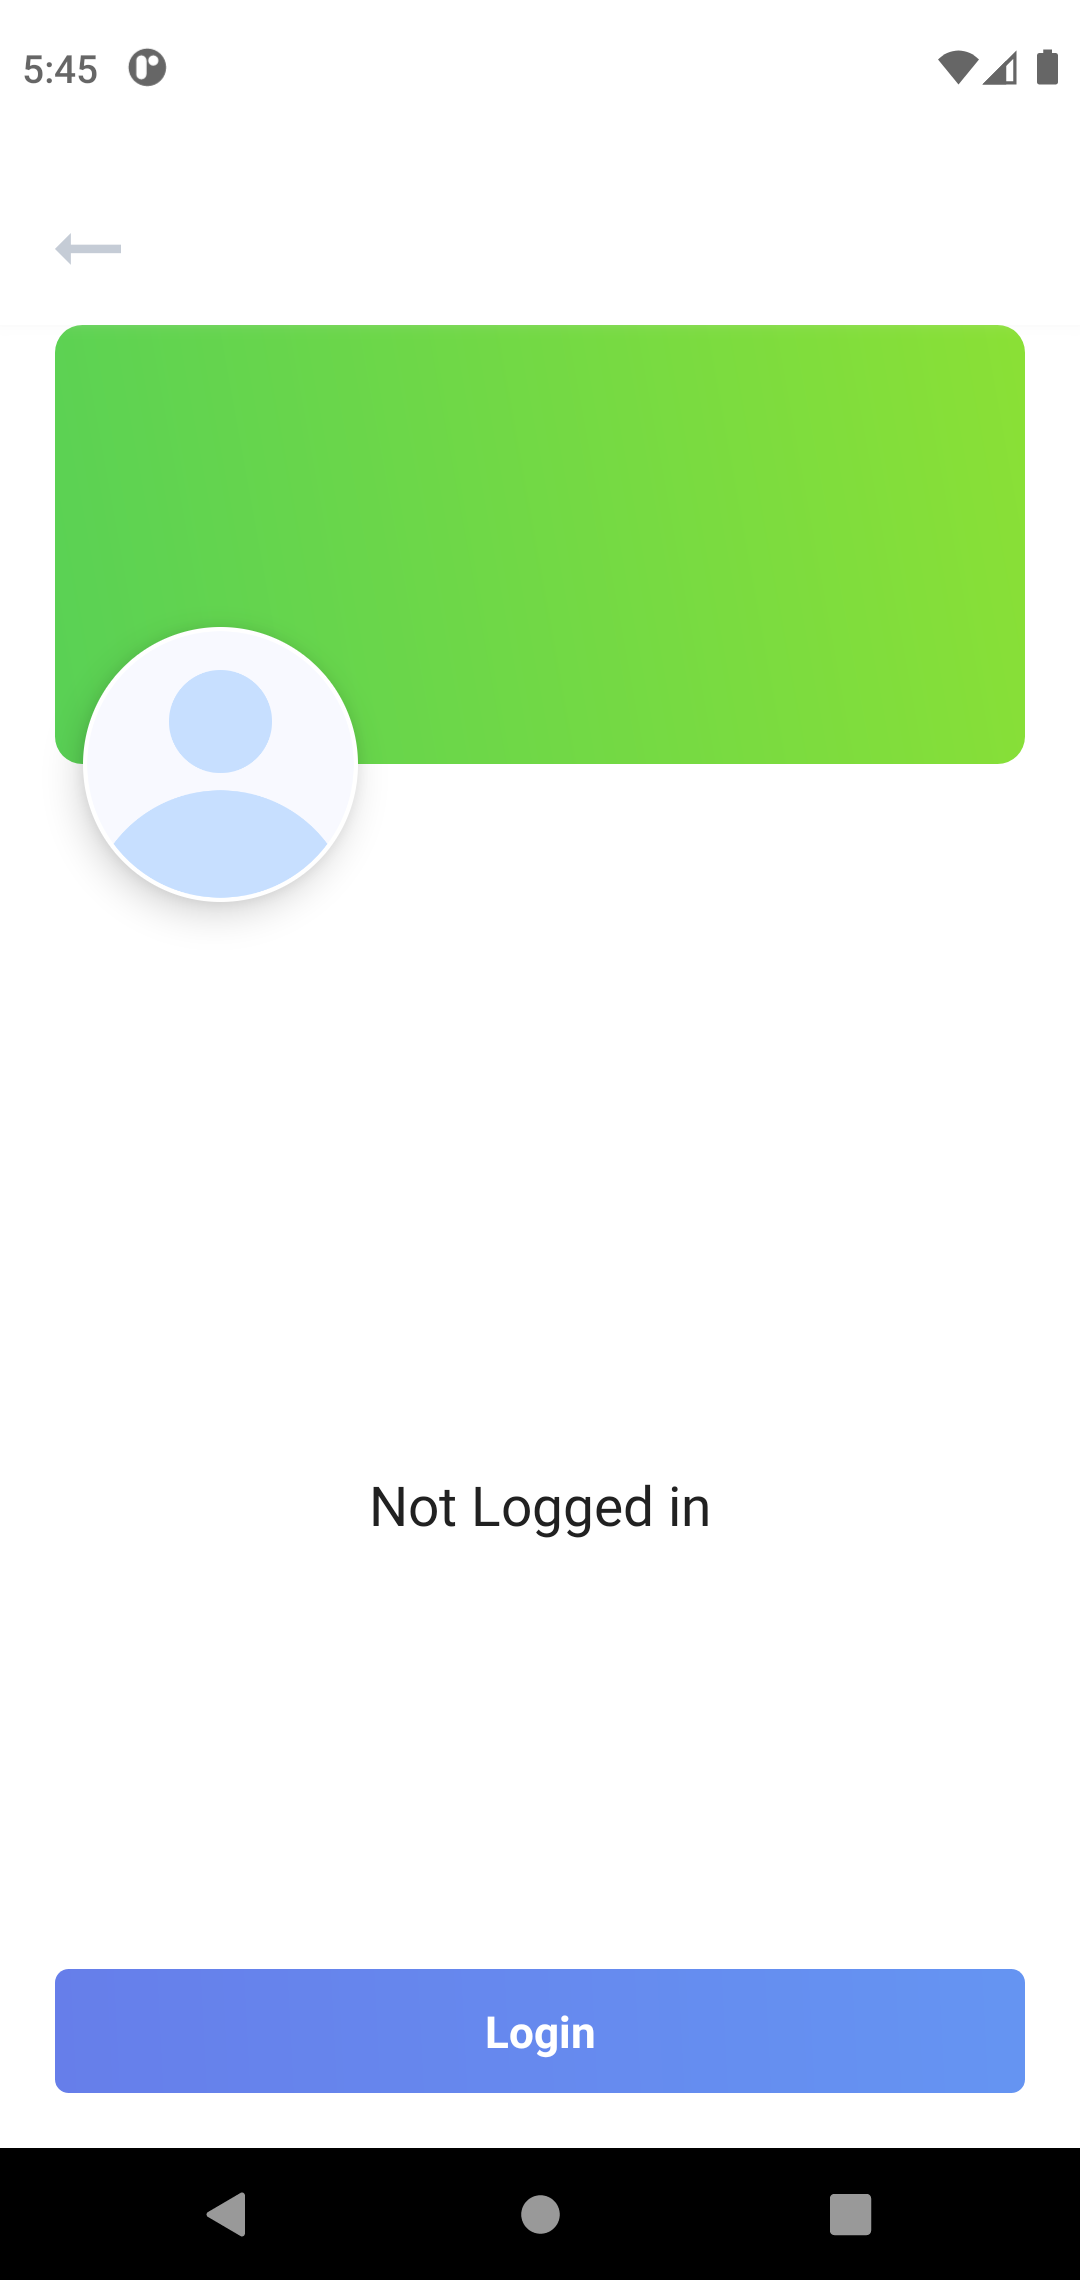
\includegraphics[scale=0.2]{figures/Testing/guest.png}}%
	\caption{Guest interaction}
\end{figure}

Everytime a button is pressed which requires user login, this screen pops up.
\newpage
\section{Usability testing}
This sort of testings makes us known whether the application is easy to use and learn by the user or not. It can only be done getting a response from potential users through testing. Since there was no contact with any potential user, Tauheed Butt asked the supervisor at his job to review the application and find any bugs and issues. Initially the font size and heights of buttons were too big. They pointed it out and it was fixed accordingly. However color scheme was highly appreciated as it wasn't too sharp on the eyes.
\section{Software performance testing}
The application relies on API calls to load data in it. If too much of that starts getting stored locally, the application will end up using a lot of user's storage. So there needs to be found a balance in between. Since tokens, roles and wish-list are being stored locally, the login and other related processes get executed quickly. They take up to max 0.1 sec to load. It also depends on what type of device is running the application. If an old device is used, its performance will degrade tremendously.
\section{Compatibility testing}
The application being cross-platform is its strong suit and it needs to be tested accordingly. The web application runs flawlessly on all type of Operating Systems. However, some browsers fail to load some image and font assets. The team failed to fix those issues.
\section{Exception handling}
Since there are 3 views to the mobile application, it is very common to run into exceptions. Some places where user's registered details are being used need to be conditionally changed to the guest's details. Many were handled during development. The API calls are done asynchronously which are bound to produce some exceptions. If not handled, the app can crash. Those ares of code were put in try catch blocks in order to prevent the application from crashing.
\section{Load testing}
The mobile version can experience great amount of load in case of re-rendering due to concurrent changes in state. Some were handled by using useEffect hook of React. Others were being caused due to being able to do API calls by pressing button again and again. This was handled by disabling the button when the API call was already in process. Once it was completed only then the button was enabled.
\section{Security testing}
The Server however can experience great amount of load in form of DDoS attacks so it needs to be catered accordingly. The access to it is the domain of the server. Where ever it gets used, it was put inside environment variable file which is automatically hidden in any project used. Even if not, it can be manually done so. Other form of load it can receive is by being able to send requests with no authentication and validation. The authentication gets handled through JWT Token which can only be generated if correct login/sign up credentials are provided. The sign up credentials are also validated on front end and back end to avoid repeated API calls.
\section{Installation testing}
Once the server was deployed to Heroku, its domain was tested using Postman. A login request was sent to it to check whether a response is returned or not. It ended up sending the response back. The mobile application was installed on android through the generated apk. It successfully installed however it prompted that the author is not trust worthy. This happens if the application is not registered with Google Play. It can cause doubt in the users who will avoid from using the application.
\newpage

\section{Testing Tables}
% Your image goes here
\noindent

\begin{table}[h]
    \centering
    \caption{TC-001}
    \begin{tabular}{ |p{3.8cm}|p{8cm}| }
        \hline
        \textbf{Test Case ID}    & TC-001                                    \\
        \hline
        \textbf{Test Case Name}  & Change in Profile                         \\
        \hline
        \textbf{Test Case Field} & User Profile                              \\
        \hline
        \textbf{Actors}          & Client, Owner                             \\
        \hline
        \textbf{Description}     & User will change their profile details    \\
        \hline
        \textbf{Pre Conditions}  & User must be logged in                    \\
        \hline
        \textbf{Input Summary}   & User enters their details in input fields \\
        \hline
        \textbf{Expected Result} & Save Button Appears                       \\
        \hline
        \textbf{Actual Result}   & Save Button did Appear                    \\
        \hline
        \textbf{Pass/Fail}       & Pass                                      \\
        \hline
    \end{tabular}
\end{table}

\begin{table}[h]
    \centering
    \caption{TC-002}
    \begin{tabular}{ |p{3.8cm}|p{8cm}| }
        \hline
        \textbf{Test Case ID}    & TC-002                                            \\
        \hline
        \textbf{Use Case ID}     & UC-018                                            \\
        \hline
        \textbf{Test Case Name}  & Send Button                                       \\
        \hline
        \textbf{Test Case Field} & User CRM                                          \\
        \hline
        \textbf{Actors}          & Client                                            \\
        \hline
        \textbf{Description}     & User will type in chat and send button will apear \\
        \hline
        \textbf{Pre Conditions}  & User must be logged in                            \\
        \hline
        \textbf{Input Summary}   & User enters text input field                      \\
        \hline
        \textbf{Expected Result} & Button changes from gallery to send               \\
        \hline
        \textbf{Actual Result}   & Button did Change                                 \\
        \hline
        \textbf{Pass/Fail}       & Pass                                              \\
        \hline
    \end{tabular}
\end{table}

\begin{table}[H]
    \centering
    \caption{TC-003}
    \begin{tabular}{ |p{3.8cm}|p{8cm}| }
        \hline
        \textbf{Test Case ID}    & TC-003                                            \\
        \hline
        \textbf{Use Case ID}     & UC-018                                            \\
        \hline
        \textbf{Test Case Name}  & Chat Bubble Time                                  \\
        \hline
        \textbf{Test Case Field} & User CRM                                          \\
        \hline
        \textbf{Actors}          & Client                                            \\
        \hline
        \textbf{Description}     & Time appears only at the last message             \\
        \hline
        \textbf{Pre Conditions}  & User must be logged in                            \\
        \hline
        \textbf{Input Summary}   & Message is sent or received                       \\
        \hline
        \textbf{Expected Result} & Time appears at the last message sent or received \\
        \hline
        \textbf{Actual Result}   & Time appeared at every message                    \\
        \hline
        \textbf{Pass/Fail}       & Fail                                              \\
        \hline
    \end{tabular}
\end{table}


\begin{table}[h]
    \centering
    \caption{TC-004}
    \begin{tabular}{ |p{3.8cm}|p{8cm}| }
        \hline
        \textbf{Test Case ID}    & TC-004                                                               \\
        \hline
        \textbf{Use Case ID}     & UC-015, UC-016, UC-017, UC-018                                       \\
        \hline
        \textbf{Test Case Name}  & Guest Actions                                                        \\
        \hline
        \textbf{Test Case Field} & Client View                                                          \\
        \hline
        \textbf{Actors}          & Client                                                               \\
        \hline
        \textbf{Description}     & Any action that requires authentication and guest user can't perform \\
        \hline
        \textbf{Pre Conditions}  & User must be logged out                                              \\
        \hline
        \textbf{Input Summary}   & An interaction that requires authentication is done.                 \\
        \hline
        \textbf{Expected Result} & Profile Screen is shown with message to tell user to log in first    \\
        \hline
        \textbf{Actual Result}   & Profile Screen did come up                                           \\
        \hline
        \textbf{Pass/Fail}       & Pass                                                                 \\
        \hline
    \end{tabular}
\end{table}

\begin{table}[h]
    \centering
    \caption{TC-005}
    \begin{tabular}{ |p{3.8cm}|p{8cm}| }
        \hline
        \textbf{Test Case ID}    & TC-005                                                     \\
        \hline
        \textbf{Use Case ID}     & TC-001, TC-002                                             \\
        \hline
        \textbf{Test Case Name}  & Email and Password Validation                              \\
        \hline
        \textbf{Test Case Field} & Login and Sign up                                          \\
        \hline
        \textbf{Actors}          & Client, Admin, Owner, Agent                                \\
        \hline
        \textbf{Description}     & Icon color will change based on email and password's value \\
        \hline
        \textbf{Pre Conditions}  & User must be on Sign in or Sign up Screen                  \\
        \hline
        \textbf{Input Summary}   & Data is entered into email and password field.             \\
        \hline
        \textbf{Expected Result} &
        On Empty Data: Icon Color is Grey  \newline
        On Incorrect Data: Icon Color is Red  \newline
        On Correct Data: Icon Color is Green                                                  \\
        \hline
        \textbf{Actual Result}   & Colors did change                                          \\
        \hline
        \textbf{Pass/Fail}       & Pass                                                       \\
        \hline
    \end{tabular}
\end{table}

\begin{table}[h]
    \centering
    \caption{TC-006}
    \begin{tabular}{ |p{3.8cm}|p{8cm}| }
        \hline
        \textbf{Test Case ID}    & TC-006                                                                          \\
        \hline
        \textbf{Use Case ID}     & UC-015                                                                          \\
        \hline
        \textbf{Test Case Name}  & Project Booking                                                                 \\
        \hline
        \textbf{Test Case Field} & Booking Flow                                                                    \\
        \hline
        \textbf{Actors}          & Client                                                                          \\
        \hline
        \textbf{Description}     & Project will not be booked again if already booked                              \\
        \hline
        \textbf{Pre Conditions}  & User must be logged in                                                          \\
        \hline
        \textbf{Input Summary}   & Booking order placed.                                                           \\
        \hline
        \textbf{Expected Result} & If already booked, the booking is not made and user is shown appropiate message \\
        \hline
        \textbf{Actual Result}   & It placed another booking                                                       \\
        \hline
        \textbf{Pass/Fail}       & Fail                                                                            \\
        \hline
    \end{tabular}
\end{table}

\begin{table}[h]
    \centering
    \caption{TC-007}
    \begin{tabular}{ |p{3.8cm}|p{8cm}| }
        \hline
        \textbf{Test Case ID}    & TC-007                                                      \\
        \hline
        \textbf{Use Case ID}     & UC-014, UC-013                                              \\
        \hline
        \textbf{Test Case Name}  & No items fetched                                            \\
        \hline
        \textbf{Test Case Field} & Loading Items                                               \\
        \hline
        \textbf{Actors}          & Client, Owner, Admin                                        \\
        \hline
        \textbf{Description}     & Application will fetch items based on the screen user is on \\
        \hline
        \textbf{Pre Conditions}  & User must be on a screen that loads some items              \\
        \hline
        \textbf{Input Summary}   & Page refreshed or loaded for first time.                    \\
        \hline
        \textbf{Expected Output} & If no items loaded, a message is displayed.                 \\
        \hline
        \textbf{Actual Result}   & No message displayed                                        \\
        \hline
        \textbf{Pass/Fail}       & Fail                                                        \\
        \hline
    \end{tabular}
\end{table}
\begin{table}[h]
	\centering
	\caption{TC-008}
	\begin{tabular}{ |p{3.8cm}|p{8cm}| }
		\hline
		\textbf{Test Case ID}    & TC-008                                                \\
		\hline
		\textbf{Use Case ID}     & TC-001, TC-002                                        \\
		\hline
		\textbf{Test Case Name}  & Failed Login/Signup                                   \\
		\hline
		\textbf{Test Case Field} & Authentication                                        \\
		\hline
		\textbf{Actors}          & Client, Owner, Admin, Agent                           \\
		\hline
		\textbf{Description}     & Error message will be showed on failed authentication \\
		\hline
		\textbf{Pre Conditions}  & User must be signed out                               \\
		\hline
		\textbf{Input Summary}   & User attempts authentication.                         \\
		\hline
		\textbf{Expected Output} & Error message displayed above submit button.          \\
		\hline
		\textbf{Actual Result}   & Error displayed                                       \\
		\hline
		\textbf{Pass/Fail}       & Pass                                                  \\
		\hline
	\end{tabular}
\end{table}


\begin{table}[h]
	\centering
	\caption{TC-009}
	\begin{tabular}{ |p{3.8cm}|p{8cm}| }
		\hline
		\textbf{Test Case ID}    & TC-009                                                                                       \\
		\hline
		\textbf{Use Case ID}     & UC-014, UC-013                                                                               \\
		\hline
		\textbf{Test Case Name}  & Extra items loading                                                                          \\
		\hline
		\textbf{Test Case Field} & Loading items                                                                                \\
		\hline
		\textbf{Actors}          & Client, Owner, Admin                                                                         \\
		\hline
		\textbf{Description}     & Error items need to be loaded when end of screen reached                                     \\
		\hline
		\textbf{Pre Conditions}  & User must be on a screen that loads some items.                                              \\
		\hline
		\textbf{Input Summary}   & End of screen reached after scrolling.                                                       \\
		\hline
		\textbf{Expected Output} & Loading icon showed while it attempts to get more items, if no more items, message is shown. \\
		\hline
		\textbf{Actual Result}   & Loader appeared                                                                              \\
		\hline
		\textbf{Pass/Fail}       & Pass                                                                                         \\
		\hline
	\end{tabular}
\end{table}
